\documentclass{article}
\usepackage{graphicx,amsmath,amssymb,url,multirow}
\usepackage{hyperref}
\usepackage{wrapfig}
\usepackage[nottoc,numbib]{tocbibind}
\setlength{\parindent}{0in}
\setlength{\parskip}{0.07in}

%\usepackage[paper=a4paper,dvips,top=1.5cm,left=1.5cm,right=1.5cm,
%    foot=1cm,bottom=1.5cm]{geometry}
\usepackage[paper=a4paper,top=3cm,left=2cm,right=2cm,bottom=3cm]{geometry}

% TITLE
\title{Moto User Documentation}
\author{Version 0.1 Beta}
\date{Copyright \textcircled{c}  2014 Sigma Power Engineering Pty Ltd}

\begin{document}
\pagestyle{plain}
\maketitle

% TABLE OF CONTENTS
\tableofcontents
\clearpage

% BODY
\section{Introduction}
\subsection{About Moto}
\textbf{Moto} is a parameter estimation tool that can be used to determine the equivalent circuit parameters of induction machines. The tool is intended for use in dynamic time-domain simulations such as stability and motor starting studies.

\textbf{Moto} is unique in that it provides a selection of the most advanced parameter estimation algorithms, which are more accurate and robust than those found in commercial power systems analysis software.

\subsection{About Sigma Power Engineering}
%\begin{wrapfigure}{l}{0.3\textwidth}
%  \begin{center}
\begin{figure}[!ht]
    
\includegraphics[width=0.28\textwidth]{./Figures/Sigma_Power.png}
\end{figure}

%  \end{center}
%\end{wrapfigure}

\textbf{Sigma Power Engineering Pty Ltd} is an electrical engineering consultancy and software developer based in Perth, Australia.

We are a small team of power systems engineers with decades of experience in the utility, hydrocarbons and mining sectors of Australia, Asia and Europe. Our primary focus is to offer the full range of power system studies services, while also supporting our clients with our software tools, project management and design engineering capabilities.

For more details, visit our website \href{http://www.sigmapower.com.au}{www.sigmapower.com.au}.

\subsection{Release Notes}
Version 0.1 Beta is a preliminary version of \textbf{Moto} that is restricted to estimating parameters for the double cage model with core losses. In future versions, single cage models and motor models without core losses will be implemented.

For any comments, suggestions or bug reports, please get in touch with us at \href{mailto:contact@sigmapower.com.au}{contact@sigmapower.com.au}.

\subsection{BSD License}
Redistribution and use in  binary form is permitted provided that the following conditions are met:

\begin{enumerate}
\item Redistributions in binary form must reproduce the above copyright notice, this list of conditions and the following disclaimer in the documentation and/or other materials provided with the distribution
\item All advertising materials mentioning features or use of this software must display the following acknowledgement: This product includes software developed by the Sigma Power Engineering Pty Ltd.
\item Neither the name of the Sigma Power Engineering Pty Ltd nor the names of its contributors may be used to endorse or promote products derived from this software without specific prior written permission.
\end{enumerate}

\subsection{Disclaimer}

THIS SOFTWARE IS PROVIDED BY SIGMA POWER ENGINEERING PTY LTD ''AS IS'' AND ANY
EXPRESS OR IMPLIED WARRANTIES, INCLUDING, BUT NOT LIMITED TO, THE IMPLIED
WARRANTIES OF MERCHANTABILITY AND FITNESS FOR A PARTICULAR PURPOSE ARE
DISCLAIMED. IN NO EVENT SHALL SIGMA POWER ENGINEERING PTY LTD BE LIABLE FOR ANY
DIRECT, INDIRECT, INCIDENTAL, SPECIAL, EXEMPLARY, OR CONSEQUENTIAL DAMAGES
(INCLUDING, BUT NOT LIMITED TO, PROCUREMENT OF SUBSTITUTE GOODS OR SERVICES;
LOSS OF USE, DATA, OR PROFITS; OR BUSINESS INTERRUPTION) HOWEVER CAUSED AND
ON ANY THEORY OF LIABILITY, WHETHER IN CONTRACT, STRICT LIABILITY, OR TORT
(INCLUDING NEGLIGENCE OR OTHERWISE) ARISING IN ANY WAY OUT OF THE USE OF THIS
SOFTWARE, EVEN IF ADVISED OF THE POSSIBILITY OF SUCH DAMAGE.

\newpage
\section{Technical Background}

\subsection{Induction Motor Equivalent Circuits}

An induction machine can be viewed as a generalised transformer with an air gap and a rotating short-circuited secondary winding. The equivalent circuit of an induction motor is therefore similar to that of a transformer. The key difference is in the rotor equivalent circuit, where the voltages and currents are proportional to the slip frequency. This is commonly represented in the equivalent circuit by a variable (slip-dependent) rotor resistance (i.e. $\frac{R_{r}}{s}$).

For balanced steady-state analysis, it is acceptable to use a per-phase equivalent circuit. Analysis is also made simpler by working with per-unit values, where the scaling factors required to calculate polyphase quantities (such as polyphase power) are not required. The general induction motor per-phase equivalent circuit with all parameters referred to the stator is shown in Figure \ref{fig:general_equiv_circuit}.

\begin{figure}[htp]
\begin{center}
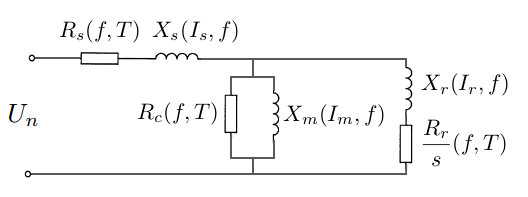
\includegraphics[scale=0.85]{./Figures/General_equiv_circuit.png}
\caption{General induction motor equivalent circuit}
\label{fig:general_equiv_circuit}
\end{center}
\end{figure}

The parameters of this equivalent circuit are as follows:

\begin{itemize}
\item  $R_{s}$ is the stator resistance (pu)
\item $X_{s}$ is the stator leakage reactance (pu)
\item $X_{m}$ is the magnetising reactance (pu) 
\item $R_{c}$ is the core loss component (pu) 
\item $X_{r}$ is the rotor leakage reactance (pu) 
\item $R_{r}$ is the rotor resistance (pu) 
\end{itemize}

The motor equivalent circuit in Figure \ref{fig:general_equiv_circuit} shows that the parameters vary with frequency / slip, current (i.e. saturation effects) and temperature, for the following reasons:

\begin{itemize}
  \item AC resistances for the copper windings are temperature dependent \cite{waters_1983}
  \item Inductances will vary due to eddy currents and saturation of teeth and core \cite{rogers_1987}
  \item Rotor resistance is frequency (slip) dependent due to eddy currents in deep rotor bars or double cage rotors \cite{boldea_2002}
  \item Impedances are affected by the skin effect at different frequencies \cite{boldea_2002}
\end{itemize}

For power system studies, it is desirable to use a motor equivalent circuit with constant parameters that are valid over the full range of motor speeds (i.e. from 0 to 1 pu). It is important to note that these parameters will not likely correspond to the real motor parameters, since as noted above, the real parameters are slip, current and temperature dependent. However, the set of constant equivalent circuit parameters will match the motor's performance characteristics over the full speed range (e.g. torque-slip and current-slip curves, power factor, efficiency, etc).

While others have attempted to apply motor models with variable parameters (for example, Haque in \cite{haque_2008}), there does not appear to be significant gains to be had by this approach and it only makes the model more complicated and less manageable for standard power systems analysis programs. Therefore, only constant parameter models are considered in Moto. In the following subsections, the two most common constant parameter equivalent circuit models are presented. 

\subsubsection{Single Cage Model}

The single cage model is simply the general equivalent circuit in Figure \ref{fig:general_equiv_circuit} with constant parameters. The single cage model is normally suitable to represent the performance characteristics of wound-rotor motors. Two single cage equivalent circuits are shown below in Figures \ref{fig:single_cage_model} and \ref{fig:single_cage_core_losses} depicting the model with and without core losses respectively. Note that in Figure \ref{fig:single_cage_core_losses}, the core loss component is lumped as a single shunt resistance placed at the input of the equivalent circuit. This is done for practical reasons as described in \cite{pedra_2008}.

\begin{figure}[htp]
\begin{center}
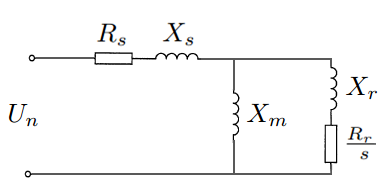
\includegraphics[scale=0.85]{./Figures/Single_cage_equiv_circuit.png}
\caption{Basic single cage model equivalent circuit (5 parameters)}
\label{fig:single_cage_model}
\end{center}
\end{figure}

\begin{figure}[htp]
\begin{center}
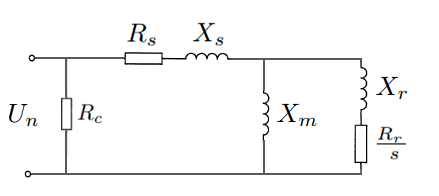
\includegraphics[scale=0.7]{./Figures/single_cage.png}
\caption{Single cage model with core losses (6 parameters)}
\label{fig:single_cage_core_losses}
\end{center}
\end{figure}

\subsubsection{Double Cage Model}

To account for the effects of double-cage rotors or deep bar rotors (e.g. most squirrel-cage machines), a second rotor branch is added to the equivalent circuit of the single cage model. Figures \ref{fig:double_cage_model} and \ref{fig:double_cage_core_losses} show the double cage model equivalen circuit with and without core losses. As in the single cage model, the core losses are represented as a single shunt resistance at the input of the equivalent circuit.

\begin{figure}[htp]
\begin{center}
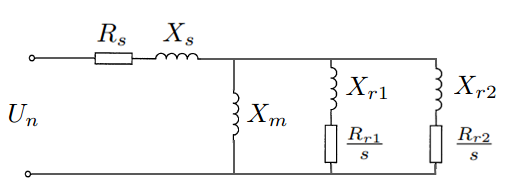
\includegraphics[scale=0.85]{./Figures/Dbl_cage_equiv_circuit.png}
\caption{Basic double cage model equivalent circuit (7 parameters)}
\label{fig:double_cage_model}
\end{center}
\end{figure}

\begin{figure}[!ht]
\begin{center}
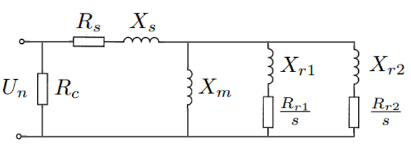
\includegraphics[scale=0.85]{./Figures/dbl_cage.png}
\caption{Double cage model with core losses (8 parameters)}
\label{fig:double_cage_core_losses}
\end{center}
\end{figure}

In the equivalent circuit, the inner cage leakage reactance $X_{r1}$ is always higher than the outer cage leakage reactance $X_{r2}$, but the outer cage impedance is typically higher than the inner cage impedance on starting. These conditions can be resolved by including the following two inequality constraints in the model \cite{pedra_2004}:

\begin{itemize}
\item $X_{r1} > X_{r2}$
\item $R_{r2} > R_{r1}$
\end{itemize}

\subsection{Calculating Torque and Current from the Equivalent Circuit}
\label{calc_torque}

The electrical torque developed in an induction machine is proportional to the square of rotor current, i.e. 

\begin{equation}
T = \frac{pq}{4 \pi f} \frac{R_{r}}{s} I_{r}^{2}
\end{equation}

\noindent where $T$ is the electrical torque developed (N-m) \\ 
\indent $p$ is the number of motor poles \\
\indent $q$ is the number of stator phases \\
\indent $f$ is the nominal frequency (Hz) \\
\indent $R_{r}$ is the equivalent rotor resistance ($\Omega$) \\
\indent $s$ is the motor slip (pu) \\
\indent $I_{r}$ is the rotor current (A)

By using per-unit values, the constant terms can be eliminated and the equation above reduces to:

\begin{equation}
T = \frac{R_{r}}{s} I_{r}^{2}
\end{equation}

where all the quantities in this equation are in per-unit values. 

It can be sees that for any given motor equivalent circuit, standard circuit analysis can be used to calculate the rotor current and therefore electrical torque. By way of example, the torque in the double cage model (without core losses) as shown in Figure \ref{fig:double_cage_model} will be calculated. 

Recasting the impedances as admittances:

\begin{eqnarray}
Y_{s} = \frac{1}{R_{s} + j X_{s}} \\
Y_{m} = \frac{1}{j X_{m}} \\
Y_{r1} = \frac{1}{\frac{R_{r1}}{s} + j X_{r1}} \\
Y_{r2} = \frac{1}{\frac{R_{r2}}{s} + j X_{r2}}
\end{eqnarray}

Applying Kirchoff's law, the voltage $U_{1}$ at the magnetising branch is:

\begin{eqnarray}
\left( U_{n} - U_{1} \right) Y_{s} = U_{1} \left( Y_{m} + Y_{r1} + Y_{r2} \right) \\
U_{n} Y_{s} = U_{1} \left( Y_{s} + Y_{m} + Y_{r1} + Y_{r2} \right) \\
U_{1} = \frac{U_{n} Y_{s}}{Y_{s} + Y_{m} + Y_{r1} + Y_{r2}}
\end{eqnarray}

The per-unit stator current $I_{s}$ is therefore:

\begin{equation}
I_{s} = \left( U_{n} - U_{1} \right) Y_{s} 
\end{equation}

The per-unit rotor currents in each cage $I_{r1}$ and $I_{r2}$ are:

\begin{eqnarray}
I_{r1} = U_{1} Y_{r1} \\
I_{r2} = U_{1} Y_{r2}
\end{eqnarray}

Finally, the per-unit electrical torque developed in the motor is:

\begin{equation}
T = \frac{R_{r1}}{s} I_{r1}^{2} + \frac{R_{r2}}{s} I_{r2}^{2}
\end{equation}

A similar kind of analysis can be done for other motor equivalent circuit models to calculate the electrical torque and current of the machine.

\subsection{Torque-Speed and Current-Speed Curves}
Based on the torque and stator current equations developed in the previous section, torque-speed and current-speed curves can be constructed from the equivalent circuit for the full range of motor speeds (i.e. from standtill to synchronous speed). 

Examples of motor torque-speed and current-speed curves are shown in Figure \ref{fig:torque-speed_curve} and Figure \ref{fig:current-speed_curve} respectively.

\begin{figure}[!htp]
\begin{center}
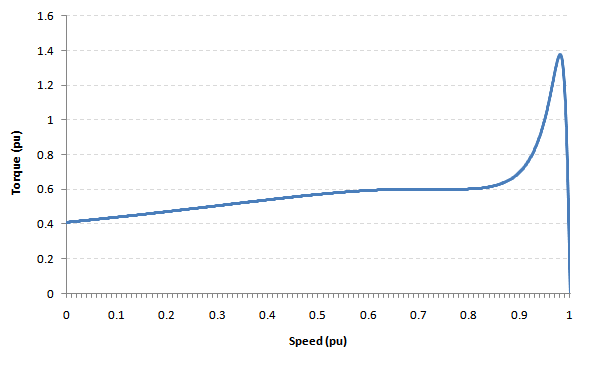
\includegraphics[scale=0.6]{Figures/torque-speed_curve.png}
\caption{Motor torque-speed curve}
\label{fig:torque-speed_curve}
\end{center}
\end{figure}

\begin{figure}[!htp]
\begin{center}
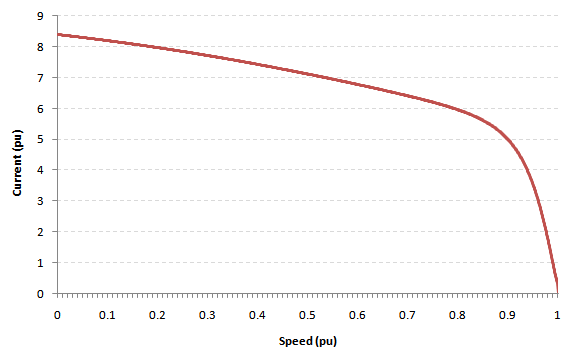
\includegraphics[scale=0.6]{Figures/current-speed_curve.png}
\caption{Motor current-speed curve}
\label{fig:current-speed_curve}
\end{center}
\end{figure}

\newpage
\subsection{Parameter Estimation Problem}

The characteristics of an induction motor are normally provided by manufacturers in the form of a standard set of performance parameters, with the following parameters being the most common:

\begin{itemize}
\item Nominal voltage, $U_n$ (V)
\item Nominal frequency, $f$ (Hz)
\item Rated asynchronous speed, $n_{fl}$ (rpm)
\item Rated (stator) current, $I_{s,fl}$ (A)
\item Rated mechanical power, $P_{m,fl}$ (kW)
\item Rated torque, $T_{n}$ (Nm)
\item Full load power factor, $\cos{\phi_{fl}}$ (pu)
\item Full load efficiency, $\eta_{fl}$ (pu)
\item Breakdown torque, $T_{b} / T_{n}$ (normalised)
\item Locked rotor torque, $T_{lr} / T_{n}$ (normalised)
\item Locked rotor current, $I_{lr} / I_{s,fl}$) (pu)
\end{itemize}

From previous sections, we know that a set of equivalent circuit parameters can yield specific torque-speed and current-speed curves. So given a set of performance parameters that contain features on the torque-speed and current-speed curves (e.g. breakdown torque, locked-rotor current, etc), is it possible to determine the corresponding equivalent circuit parameters that yield these features? This is the crux of the parameter estimation problem and can be posed as follows - "How can the motor performance parameters be converted into equivalent circuit parameters?".

While all of the performance parameters in the above set can be used in an estimation procedure, there are actually only six indpendent magnitudes that can be formed from them: $P_{m,fl}$, $Q_{fl}$, $T_{b}$, $T_{lr}$, $I_{lr}$ and $\eta_{fl}$ \cite{pedra_2004}. These independent magnitudes will thus form the basis of the problem formulation, where the independent magnitudes calculated from the equivalent circuit are matched with the performance parameters supplied by the manufacturer.

The basic double cage model shown in Figure \ref{fig:double_cage_model} is used to illustrate how these six independent magnitudes can be calculated from the equivalent circuit model. Stator and rotor currents at slip $s$ can be readily calculated from the equivalent circuit as shown in section \ref{calc_torque}.

Quantities for per-unit active power $P$, reactive power $Q$ and power factor $\cos{\phi}$ at slip $s$ can be calculated as follows:

\begin{eqnarray}
S(s) = U_{n} I_{s}(s)^{*} \\
P(s) = T(s) (1 - s) \\
Q(s) = \Im \{ S(s) \} \\
\cos{\phi} (s) = \frac{\Re \{ S(s) \}}{|| S(s) ||}
\end{eqnarray}

Nominal speed $n_{s}$ and full load slip $s_{f}$ is calculated as follows:

\begin{eqnarray}
n_{s} = \frac{120f}{p} \\
s_{f} = 1 - \frac{n_{fl}}{n_s}
\end{eqnarray}

\noindent where \indent $p$ is the number of motor poles \\
\indent $f$ is the nominal frequency (Hz) \\
\indent $n_{fl}$ is the asynchronous speed at full load (rpm)

Calculating the slip at maximum torque $s_{max}$ is found by solving the equation:

\begin{equation}
\frac{dT}{ds} = 0
\end{equation}

(Under the condition that the second derivative $\frac{d^{2}}{ds^{2}} < 0$) 

In the double cage model, the solution to this equation is not trivial and it is more convenient to use an estimate, e.g. based on an interval search between $s=0$ and $s=0.5$.

\subsection{Problem Formulation Ignoring Core Losses}
\label{sec:problem_formulation}

\subsubsection{Single Cage Model (Ignoring Core Losses)}
In the single cage model, the locked rotor torque $T_{lr}$ and locked rotor current $I_{lr}$ are not used because the single cage model does not have enough degrees of freedom to capture both the starting and breakdown torque characteristics without introducing significant errors \cite{pedra_2006}. As a result, it is more commonplace to only consider the breakdown torque $T_{b}$ in the single cage model and simply ignore the torque and current characteristics at locked rotor. For wound-rotor motors, this yields sufficiently accurate results (i.e. in terms of the resulting torque-speed curve). However, a single-cage model is unable to accurately model the torque-speed characteristics of squirrel cage motors, especially those with deep bars, and thus a double cage model should be used for these types of motors.

Without taking into account core losses, the full load motor efficiency $\eta_{fl}$ also cannot be used (see section \ref{formulation_core_losses} for more details). Therefore, there are only three independent parameters that can be used in the problem formulation: $P_{m,fl}$, $Q_{fl}$ and $T_{b}$.

These independent parameters can be used to formulate the parameter estimation in terms of a non-linear least squares problem, with a set of non-linear equations of the form $\mathbf{F}(\mathbf{x}) = \mathbf{0}$:

\begin{eqnarray}
f_{1} (\mathbf x) = P_{m,fl} - P(s_{f}) = 0 \\
f_{2} (\mathbf x) = \sin{\phi} - Q(s_{f})  = 0 \\
f_{3} (\mathbf x) = T_{b} - T(s_{max}) = 0 \\
\end{eqnarray}

\noindent where $\mathbf{F} = ( f_1, f_2, f_3 )$ and \\ 
\indent $\mathbf{x} = ( R_s, X_s, X_m, R_{r}, X_{r} )$ are the equivalent circuit parameters of the single cage model

\subsubsection{Double Cage Model (Ignoring Core Losses)}
In the double cage model, the locked rotor torque $T_{lr}$ and locked rotor current $I_{lr}$ are included as independent parameters. As in the single cage model, the full load motor efficiency $\eta_{fl}$ cannot be used without taking into account core losses. Therefore, there are five independent parameters and the following non-linear least squares problem:

\begin{eqnarray}
f_{1} (\mathbf x) = P_{m,fl} - P(s_{f}) = 0 \\
f_{2} (\mathbf x) = \sin{\phi} - Q(s_{f})  = 0 \\
f_{3} (\mathbf x) = T_{b} - T(s_{max}) = 0 \\
f_{4} (\mathbf x) = T_{lr} - T(s=1) = 0 \\
f_{5} (\mathbf x) = I_{lr} - I(s=1) = 0 \\
\end{eqnarray}

\noindent where $\mathbf{F} = ( f_1, f_2, f_3, f_4, f_5 )$ and \\ 
\indent $\mathbf{x} = ( R_s, X_s, X_m, R_{r1}, X_{r1}, R_{r2}, X_{r2} )$ are the equivalent circuit parameters of the double cage model

\subsection{Problem Formulation Considering Core Losses}
\label{formulation_core_losses}

It was previously noted that without taking into account the core (and mechanical) losses, the motor full load efficiency $\eta_{fl}$ cannot be used as an independent parameter in the problem formulation. This is because efficiency is calculated based on the ratio of output mechanical power to input electrical power. If the heat losses through the core and rotor frictional losses are not taken into account, then the equivalent circuit is not suitable to accurately estimate motor efficiency \cite{haque_2008}. It follows that attempting to use the motor full load efficiency in the estimation of the equivalent circuit without a core loss component would cause errors in the parameter estimates (e.g. the stator resistance would be overestimated). 

When core losses are included in the model, then the motor full load efficiency $\eta_{fl}$ can also be used as an independent parameter. The problem formulations are restated below for the single cage and double cage models with core losses taken into account. 

\subsection{Single Cage Model (with Core Losses)}

The non-linear least squares problem for the single cage model with core losses is as follows:

\begin{eqnarray}
f_{1} (\mathbf x) = P_{m,fl} - P(s_{f}) = 0 \\
f_{2} (\mathbf x) = \sin{\phi} - Q(s_{f})  = 0 \\
f_{3} (\mathbf x) = T_{b} - T(s_{max}) = 0 \\
f_{4} \mathbf (x) = \eta{fl} - \eta(s_{f}) = 0
\end{eqnarray}

\noindent where $\mathbf{F} = ( f_1, f_2, f_3, f_4 )$ and \\ 
\indent $\mathbf{x} = ( R_s, X_s, X_m, R_{r}, X_{r}, R_{c} )$ are the equivalent circuit parameters of the single cage model (with core losses)

\subsubsection{Double Cage Model (with Core Losses)}

The non-linear least squares problem for the double cage model with core losses is as follows:

\begin{eqnarray}
f_{1} (\mathbf x) = P_{m,fl} - P(s_{f}) = 0 \\
f_{2} (\mathbf x) = \sin{\phi} - Q(s_{f})  = 0 \\
f_{3} (\mathbf x) = T_{b} - T(s_{max}) = 0 \\
f_{4} (\mathbf x) = T_{lr} - T(s=1) = 0 \\
f_{5} (\mathbf x) = I_{lr} - I(s=1) = 0 \\
f_{6} \mathbf (x) = \eta{fl} - \eta(s_{f}) = 0
\end{eqnarray}

\noindent where $\mathbf{F} = ( f_1, f_2, f_3, f_4, f_5, f_6 )$ and \\ 
\indent $\mathbf{x} = ( R_s, X_s, X_m, R_{r1}, X_{r1}, R_{r2}, X_{r2}, R_{c} )$ are the equivalent circuit parameters of the double cage model (with core losses)

\section{Parameter Estimation Algorithms}
\label{sec:algorithms}

The parameter estimation problems formulated in the preceding sections can be solved by a variety of non-linear least squares solver algorithms. As with all non-linear least squares problems, closed form solutions are generally not available and iterative algorithms are used to converge on a solution by minimising error residuals.

Motor parameter estimation algorithms generally fall under three broad classes:
\begin{enumerate}
\item \textbf{Descent Methods}: are the class of algorithms based on variations of Newton's method for convergence to a solution, e.g. Newton-Raphson, Levenberg-Marquardt, etc
\item \textbf{Natural Optimisation Methods}: are the class of algorithms based on processes found in nature where successive randomised trials are filtered for "fitness" at each iteration, e.g. genetic algorithm, particle swarm optimisation, ant colony optimisation, simulated annealing, etc
\item \textbf{Hybrid Methods}: are the class of algorithms that use a combination of both descent and natural optimisation methods. 
\end{enumerate}

\textbf{Moto} provides the following seven (7) algorithms for solving parameter estimation algorithms:

\begin{itemize}
\item Newton-Raphson (Descent)
\item Levenberg-Marquardt (Descent)
\item Damped Newton-Raphson (Descent)
\item Genetic Algorithm (Natural Optimisation)
\item GA-NR (Hybrid)
\item GA-LM (Hybrid)
\item GA-DNR (Hybrid)
\end{itemize}

\subsection{Newton-Raphson Algorithm}
\label{sec:nr_algo}
Of the class of descent methods used to solve non-linear least squares problems, the Newton-Raphson (NR) algorithm is probably the most straightforward. The NR algorithm is an iterative method where each iteration is calculated as follows:

\begin{equation}
\label{eqn_NR}
\boldsymbol{x}^{k+1} = \boldsymbol{x}^{k} - h_{n} \mathbf{J}^{-1}  \mathbf{F}( \boldsymbol{x}^{k})
\end{equation}

where $\boldsymbol{x}^{k+1}$ is the solution at the $(k+1)$th iteration, $\boldsymbol{x}^{k}$ is the solution at the $k$th iteration, $h_{n}$ is the step-size coefficient (more on this later) and $\mathbf{J}$ is the Jacobian matrix evaluated with the parameters at the $k$th iteration, $\boldsymbol{x}^{k}$.

The Jacobian matrix $\mathbf{J}$ has the general form:

\begin{equation}
\label{eqn_Jac}
\mathbf{J} = \left( \begin{array}{ccc}
\frac{\partial f_{1}}{\partial x_{1}}  & \ldots & \frac{\partial f_{1}}{\partial x_{6}} \\
\vdots & \ddots & \vdots \\
\frac{\partial f_{6}}{\partial x_{1}}  & \ldots & \frac{\partial f_{6}}{\partial x_{6}} \\ \end{array} \right)
\end{equation}

For systems where it is impractical to compute the exact partial derivatives analytically, a numerical approximation may be used with finite difference equations:

\begin{equation}
\frac{\partial f_{i}}{\partial x_{j}} \approx \frac{f_{i} (\mathbf{x} + \boldsymbol{\delta_{j}} h) - f_{i} (\mathbf{x})}{h}
\end{equation}

where $\boldsymbol{\delta_{j}}$ is vector of zeros with a single non-zero value of 1 at the j-th element and $h$ is a constant with a very small absolute value (e.g. $1 \times 10^{-6}$).

\begin{figure}
\begin{center}
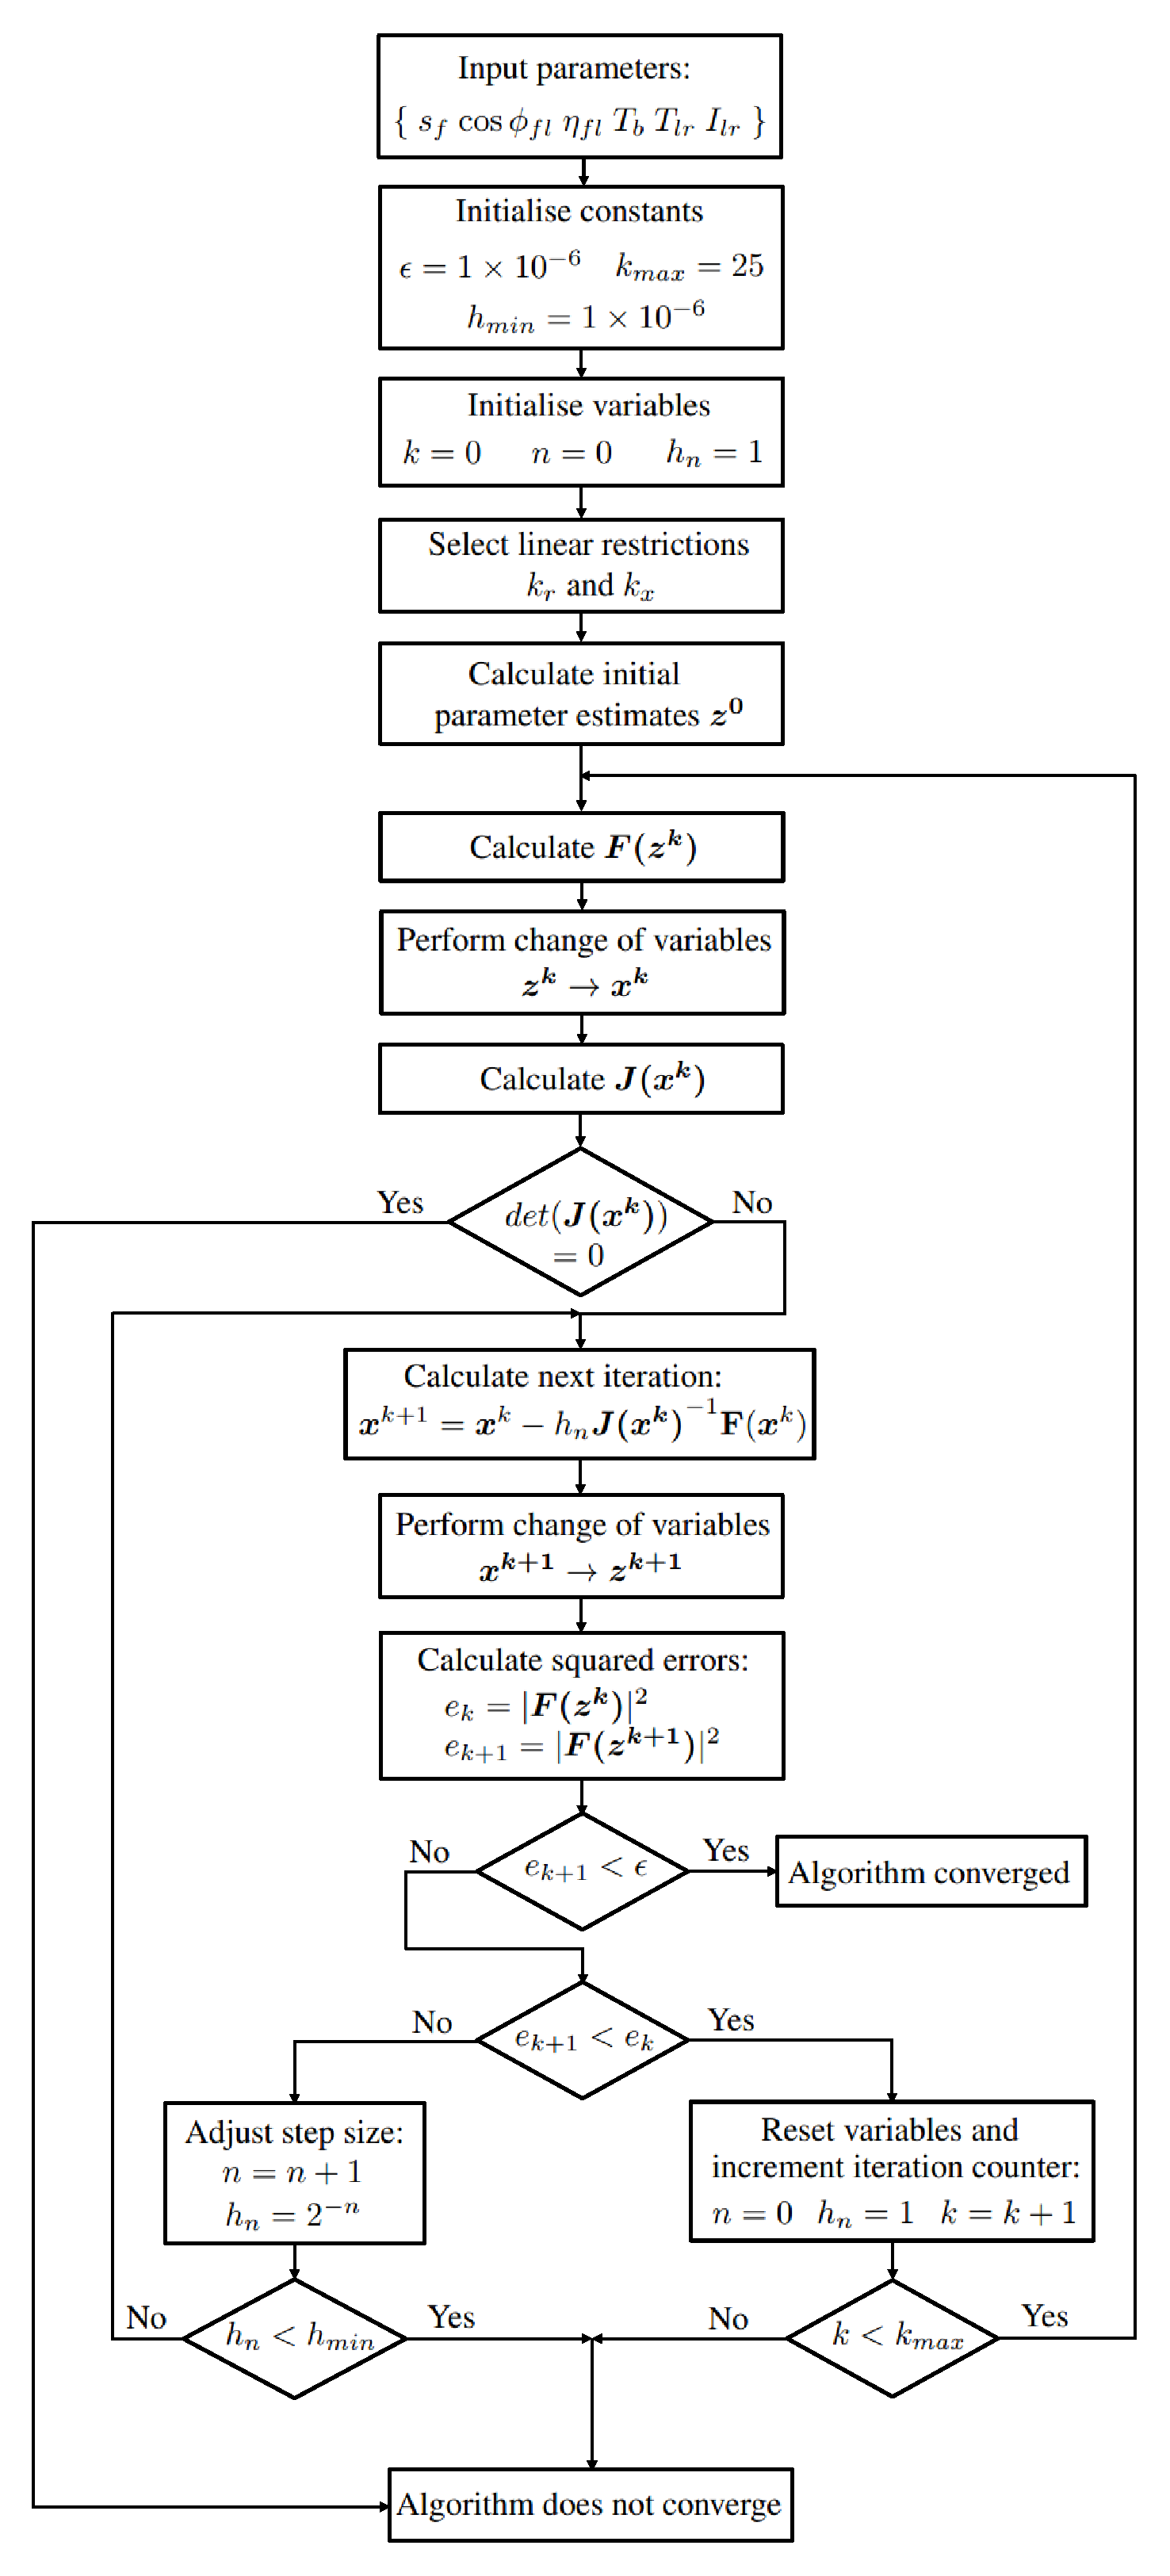
\includegraphics[scale=0.42]{./Figures/Algo_Flowchart.pdf}
\caption{Flowchart for conventional NR algorithm}
\label{fig:algo_flowchart}
\end{center}
\end{figure}

A modified form of the NR algorithm proposed in \cite{pedra_2008} for the double cage model is shown in Figure \ref{fig:algo_flowchart}. This algorithm was selected because of its completeness, numerical accuracy and robustness compared to previously proposed methods (for example, in \cite{johnson_1991}, \cite{rogers_1987} and \cite{waters_1983}). Furthermore, the algorithm can be applied using commonly available manufacturer data, whereas other algorithms require more detailed data that may not be readily available (for example, the full torque-speed curve in \cite{lindenmeyer_2001}). Two other features of the algorithm that aid its robustness are worth highlighting:

\subsubsection{Need for Linear Constraints}
\label{sec:linear_constraints}

It can be seen from the problem formulations in the previous chapter that in each case, the number of paramters to be estimated (i.e. unknown variables) exceeds the number of simultaneous equations. In other words, the systems of equations are all underdetermined. Therefore, in order to make the systems exactly determined and solvable with descent algorithms such as the NR algorithm, we must either:

\begin{enumerate}
\item Fix two parameters a priori (i.e. parameters are "known")
\item Impose two constraints on the problem formulations, e.g. linear constraints

\end{enumerate}

The use of linear constraints was found to be superior to fixed parameters and therefore, the descent algorithms in \textbf{Moto} include two linear restrictions by default. 

It was shown in \cite{pedra_2004} that the stator resistance $R_{s}$ was the least sensitive parameter in the equivalent circuit, i.e. variations in the value of $R_{s}$ had the least significant effect on the resulting torque-speed and current-speed curves. Therefore, $R_{s}$ can be subject to a linear restriction by linking it to the rotor resistance, leading to the first linear constraint:

\begin{itemize}
\item $R_{s} = k_{r} R_{r}$ (for the single cage model)
\item $R_{s} = k_{r} R_{r1}$ (for the double cage model)
\end{itemize}

\noindent Where $k_{r}$ is a constant linear constraint

Moreover, it is assumed that the rotor reactance is linearly related to the stator reactance, leading to the second linear constraint. 

\begin{itemize}
\item $X_{r} = k_{x} X_{s}$ (for the single cage model)
\item $X_{r2} = k_{x} X_{s}$ (for the double cage model)
\end{itemize}

\noindent Where $k_{x}$ is a constant linear constraint

\subsubsection{Parameter Constraints}
\label{sec:constraints}
The inequality constraints of the double cage model ($X_{r1} > X_{r2}$ and $R_{r2} > R_{r1}$) can be implicitly included into the formulation by a simple change of variables \cite{pedra_2004}:

\begin{eqnarray*}
x_{1} = R_{r1} \\
x_{2} = R_{r2} - R_{r1} \\
x_{3} = X_{m} \\
x_{4} = X_{s} \\
x_{5} = X_{r1} - k_{x} X_{s} \\
x_{6} = R_{c} \\
\end{eqnarray*}

Furthermore, only the absolute values of the parameter estimates are used to ensure that no negative parameters are estimated.

\subsubsection{Adaptive Step Size}

The step size $h_{n}$ in equation \ref{eqn_NR} is a scaling term that determines how far the algorithm should go along the descent direction $\mathbf{J}^{-1}  \mathbf{F}( \boldsymbol{x}^{k})$. Choosing a step size that is too large risks the algorithm not converging. On the other hand, choosing a step size that is too small can cause the algorithm to converge too slowly. An adaptive step size can avoid both these problems by starting with a high step size and only reducing it if the algorithm does not converge (refer to the flowchart in Figure \ref{fig:algo_flowchart}).

\subsubsection{Initial Conditions}
\label{sec:base_init}
For the base case NR algorithm, the initial parameter estimates are selected as follows \cite{pedra_2004}:

\begin{eqnarray*}
\label{init_conditions}
R_{r1} = \frac{U_{n} s_{f}}{P_{m,fl}} \\
X_{m} = \frac{U_{n}}{Q_{fl}} \\
X_{s} = 0.05 X_{m} \\
R_{s} = k_{r} R_{r1} \\
R_{r2} = 5 R_{r1} \\
X_{r1} = 1.2 X_{s} \\
X_{r2} = k_{x} X_{s} \\
R_{c} = 10
\end{eqnarray*}

%----------------------------------------------------------------------------------------
%	LM ALGORITHM
%----------------------------------------------------------------------------------------

\subsection{Levenberg-Marquardt Algorithm}
The Levenberg-Marquardt (LM) algorithm, sometimes called the damped least-squares algorithm, is another popular technique for solving least-saures problems \cite{levenberg_1944} \cite{marguardt_1963}. In the LM algorithm, each iteration is calculated as follows:

\begin{equation}
\label{eqn_LM}
\boldsymbol{x}^{k+1} = \boldsymbol{x}^{k} -  \left[ \mathbf{J}^{T} \mathbf{J} + \lambda \, \mathbf{diag}(\mathbf{J}^{T}\mathbf{J}) \right]^{-1} \mathbf{J}^{T} \mathbf{F}(\boldsymbol{x}^{k})
\end{equation}

where $\boldsymbol{x}^{k+1}$ is the solution at the $(k+1)$th iteration, $\boldsymbol{x}^{k}$ is the solution at the $k$th iteration, $\lambda$ is the damping parameter (more on this later) and $\mathbf{J}$ is the Jacobian matrix evaluated with the parameters at the $k$th iteration, $\boldsymbol{x}^{k}$ (as described previously in Equation \ref{eqn_Jac}).

Parameter constraints as implemented in the Newton-Raphson algorithm are also applied in the LM algorithm (refer to Section \ref{sec:constraints}). The initial conditions are also selected in the same way as the NR algorithm.

The selection of the damping parameter $\lambda$ affects both the direction and magnitude of an iteration step. If the damping parameter is large, then the algorithm will move at short steps in the steepest descent direction. This is good when the present iteration is far away from the solution. On the other hand, if the damping parameter is small, then the algorithm approaches a Gauss-Newton type method, which exhibits good convergence in the neighbourhood of the solution.

Therefore, the damping parameter should be updated at each iteration depending on whether the algorithm is far or close to the solution. The "gain ratio" method suggested  for adjusting the damping factor by Marquardt in \cite{marguardt_1963}was not found to be effective in induction motor problems. Therefore, \textbf{Moto} uses a damping factor adjustment method based only on the error term (i.e. the numerator of the gain ratio). 

The damping parameter is updated as follows:

\begin{equation}
\lambda =
\begin{cases}
\lambda \times \beta, & \text{if } \mathbf{F}(\boldsymbol{x}^{k}) - \mathbf{F}(\boldsymbol{x}^{k+1}) < 0 \\
\frac{\lambda}{\gamma}, & \text{if } \mathbf{F}(\boldsymbol{x}^{k}) - \mathbf{F}(\boldsymbol{x}^{k+1}) > 0
\end{cases}
\end{equation}

Where $\beta$ and $\gamma$ are algorithm control parameters. In \textbf{Moto}, the algorithm control parameters are $\beta = 3$ and $\gamma = 3$.

%----------------------------------------------------------------------------------------
%	DAMPED NR ALGORITHM
%----------------------------------------------------------------------------------------

\subsection{Damped Newton-Raphson Algorithm}
The damped Newton-Raphson algorithm is a variation of the conventional NR algorithm where a damping factor is applied to help get around problems with near-singular and/or ill-conditioned Jacobian matrices. In the damped NR algorithm, each iteration is calculated as follows:

\begin{equation}
\label{eqn_DNR}
\boldsymbol{x}^{k+1} = \boldsymbol{x}^{k} - h_{n} (\mathbf{J}^{-1} + \lambda I ) \mathbf{F}( \boldsymbol{x}^{k})
\end{equation}

Where the damping parameter $\lambda$ is adjusted at each iteration based on the error term as follows:

\begin{equation}
\lambda =
\begin{cases}
\lambda \times \beta, & \text{if } \mathbf{F}(\boldsymbol{x}^{k}) - \mathbf{F}(\boldsymbol{x}^{k+1}) < 0 \\
\frac{\lambda}{\gamma}, & \text{if } \mathbf{F}(\boldsymbol{x}^{k}) - \mathbf{F}(\boldsymbol{x}^{k+1}) > 0
\end{cases}
\end{equation}

Where $\beta$ and $\gamma$ are algorithm control parameters. In \textbf{Moto}, the algorithm control parameters are $\beta = 3$ and $\gamma = 3$.

All other aspects of the damped NR algorithm are the same as per the conventional NR algorithm described in Section \ref{sec:nr_algo} (e.g. parameter constraints, adaptive step sizes, etc)

\subsection{Genetic Algorithm}
\label{sec:genetic_algo}
The genetic algorithm (GA) is part of the class of evolutionary algorithms modelled on natural selection and evolutionary processes to optimise non-linear cost functions. It was developed in the 1960s and 1970s, but only gained widespread popularity in the late 1980s when advances in computational processing power made the algorithm more practical to apply on desktop computers \cite{haupt_1998}. 

The goal of the genetic algorithm is to minimise a non-linear cost function. For non-linear least squares problems, this can be interpreted as minimising the squared error residuals. The general methodology can be summarised under four broad headings - 1) Initialisation, 2) Fitness and Selection, 3) Breeding and Inheritance and 4) Termination.

\begin{enumerate}
\item \textbf{Initialisation}: an initial population of candidate solutions to minimise the cost function is first generated, typically via random sampling. The size of the population is an algorithm setting and largely depends on the nature of the problem.

\item \textbf{Fitness and Selection}: the population is ranked according to the fitness of its members. The fitness of each member is normally calculated from the cost function, where lower values signal higher fitness. The fittest set of members are selected to evolve / breed the next generation.

\item \textbf{Breeding and Inheritance}: the members chosen in the selection stage are designated as "parents" and evolved to create the next generation of candidate solutions ("children"). There are three common methods for generating children - elite children, crossover and mutation.

Elite children are simply clones of the fittest-ranked parents. In the crossover operation, pairs of parents are bred together by randomly selecting traits from each parent that are passed on to the children. In the mutation operation, the traits of a parent are randomly altered (mutated) and then passed on to the children. Crossover and mutation are obviously inspired by nature and in the genetic algorithm, they can either be implemented simultaneously or as separate processes.

\item \textbf{Termination}: once the next generation of candidate solutions has been produced, the population is then ranked again according to their fitness. Since the least fit members of the previous generation have been discarded, the average fitness of the new generation should be higher. Successive generations are bred until either a converging solution is found (i.e. a squared error $<1 \times 10^{-5}$) or the maximum number of generations is reached.

\end{enumerate}

In the context of motor parameter estimation, the genetic algorithm is used to minimise the squared error of the problem formulation vector $\mathbf{F}$. In GA terminology, the squared error is the fitness function and is calculated as follows:

\begin{equation}
fitness = \mathbf{F} \mathbf{F}'
\end{equation}

\noindent where $\mathbf{F} = ( f_1, f_2, f_3, f_4, f_5, f_6 )$

Genetic algorithms can be binary coded where the solution paramaters are quantized into binary strings (for example, in \cite{nangsue_1999}, \cite{weatherford_2003} and \cite{nolan_1994}). However, the equivalent circuit parameters in a motor are continuous parameters and not naturally quantized. Thus, binary coding necessarily imposes limits on the precision of the parameters (i.e. due to the chosen length of the binary string). For this reason, a continuous parameter algorithm is used instead.

An initial population of $n_{pop}$ parameter estimates are randomly sampled from a uniform distribution with upper and lower limits as shown in Table \ref{tab:ga_range}.

\begin{table*}[htp]
	\renewcommand{\arraystretch}{1.3}
	\begin{center}
	\begin{tabular}{|c|c|c|}
        \hline
		  \multirow{2}{*}{Parameter} & \multicolumn{2}{|c|}{Range of Initial Estimate (pu)} \\ \cline{2-3}
        & Lower Bound & Upper Bound \\ \hline
        $R_{s}$  	& 0  & 0.15	\\ \hline
        $X_{s}$  	& 0  & 0.15	\\ \hline
        $X_{m}$  	& 0  & 5	\\ \hline
        $R_{r1}$  	& 0  & 0.15	\\ \hline
        $X_{r1}$  	& 0  & 0.30	\\ \hline
        $R_{r2}$  	& 0  & 0.15	\\ \hline
        $X_{r2}$  	& 0  & 0.15	\\ \hline
        $R_{c}$  	& 0  & 100	\\ \hline
    \end{tabular}
	\caption{Range of initial parameter estimates}
	\label{tab:ga_range}
	\end{center}
\end{table*}

The fitness of each member in the population is then calculated and ranked. The lowest fitness members are discarded and the rest are retained to form the mating pool for the next generation (there are $n_{pool}$ members in the mating pool).

The fittest $n_{e}$ members in the mating pool are retained for the next generation as \textbf{elite children}. 

Of the remaining $n_{pop} - n_{e}$ children to be created for the next generation, $c_{f}$\% will be produced by crossover and the rest ($1 - c_{f}$\%) by mutation. The proportion $c_{f}$ is called the \textbf{crossover fraction}.

\begin{enumerate}

\item \textbf{Crossover}: in the crossover process, two members of the mating pool are randomly selected and combined by taking a random blend of each member's parameters, e.g. the crossover of parameter $R_{s}$:

\begin{equation}
	R_{s, child} = \alpha R_{s, parent 1} + (1 - \alpha) R_{s, parent 2}
\end{equation}

\noindent where $\alpha$ is a random variable selected from a uniform distribution over the interval $[0,1]$

\item \textbf{Mutation}: in the mutation process, a member of the mating pool is randomly selected and its parameters are mutated by adding Gaussian noise with parameter-dependent standard deviations (see Table \ref{tab:ga_mutation}).

\end{enumerate}

\begin{table*}[htp]
	\renewcommand{\arraystretch}{1.3}
	\begin{center}
	\begin{tabular}{|c|c|}
        \hline
		  Parameter & Standard Deviation ($\sigma$) \\ \hline
        $R_{s}$  	& 0.01  	\\ \hline
        $X_{s}$  	& 0.01  	\\ \hline
        $X_{m}$  	& 0.33 	\\ \hline
        $R_{r1}$  	& 0.01  \\ \hline
        $X_{r1}$  	& 0.01  	\\ \hline
        $R_{r2}$  	& 0.01  	\\ \hline
        $X_{r2}$  	& 0.01  	\\ \hline
        $R_{c}$  	& 6.67  	\\ \hline
    \end{tabular}
	\caption{Standard deviations for mutation noise}
	\label{tab:ga_mutation}
	\end{center}
\end{table*}

The fitness of the next generation is then calculated and the process repeats itself for $n_{gen}$ generations.

The default settings for the genetic algorithm implemented in \textbf{Moto} for motor parameter estimation are shown in Table \ref{tab:ga_default}. A flowchart of the genetic algorithm implemented in \textbf{Moto} is shown in Figure \ref{fig:ga_algorithm}.

\begin{table*}[htp]
	\renewcommand{\arraystretch}{1.3}
	\begin{center}
	\begin{tabular}{|c|c|c|}
        \hline
        Setting  	& Setting Description  & Default Value	\\ \hline
        $n_{pop}$  	& Population of each generation  & 20	\\ \hline
        $n_{pool}$  	& Number of members in the mating pool  & 15 \\ \hline
        $n_{e}$  	& Number of elite children  & 2	\\ \hline
        $c_{f}$  	& Crossover fraction  & 80\%	\\ \hline
        $n_{gen}$  	& Maximum number of generations  & 30	\\ \hline
    \end{tabular}
	\caption{Default settings for genetic algorithm}
	\label{tab:ga_default}
	\end{center}
\end{table*}

\begin{figure}
\begin{center}
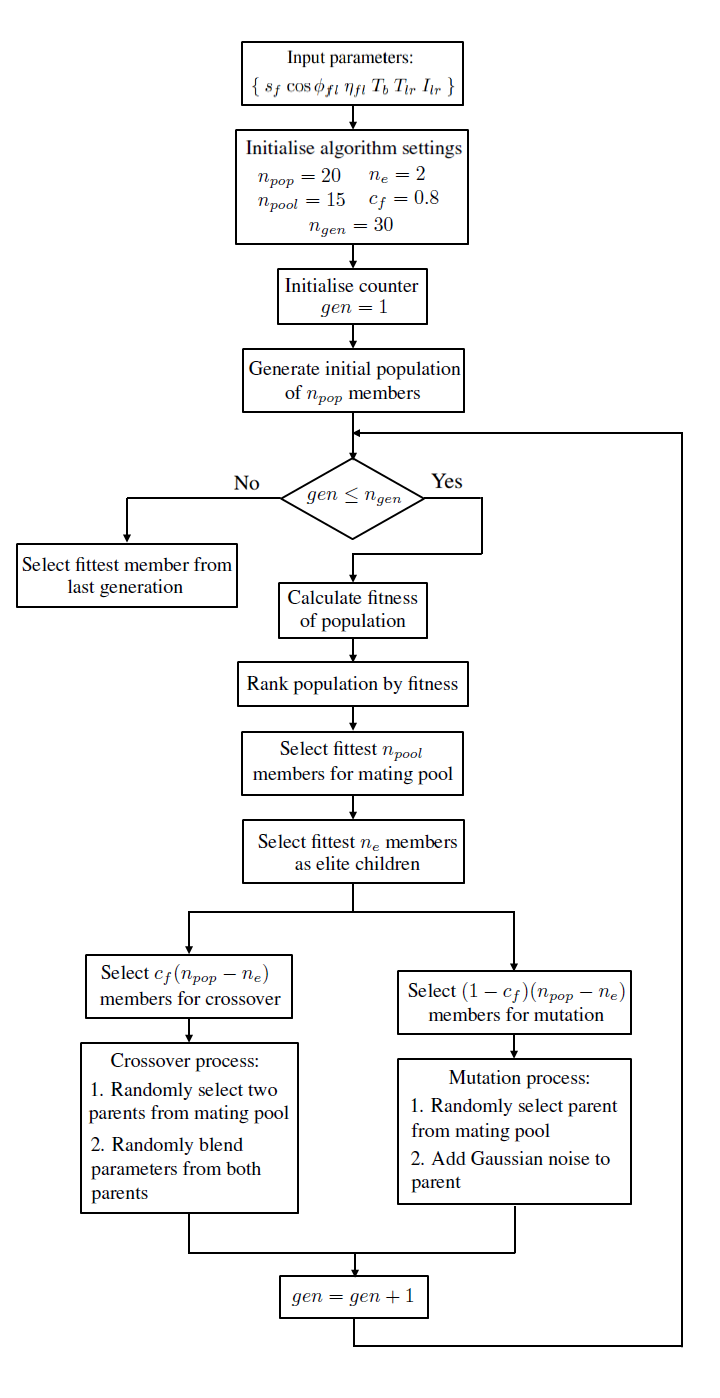
\includegraphics[scale=0.54]{./Figures/GA_Algorithm.png}
\caption{Flowchart for genetic algorithm}
\label{fig:ga_algorithm}
\end{center}
\end{figure}

\subsection{Hybrid Algorithms}
It was shown in \cite{susanto_2013} that linear restrictions imposed on $R_s$ and $X_{r2}$ have a significant influence on the convergence and error rates of descent algorithms. The parameters $R_s$ and $X_{r2}$  are also difficult to estimate accurately based solely on commonly available manufacturer data. Moreover, the selection of initial conditions can also affect the performance of descent algorithms.

On the other hand, natural optimisation algorithms can yield lower average error rates, but never low enough to qualify for convergence (as defined by a squared error of $<1 \times 10^{-5}$). However, the performance of natural optimisation algorithms is unaffected by the choice of initial conditions.

Hybrid algorithms attempt to overcome the limitations of descent algorithms by applying a genetic algorithm to select $R_s$ and $X_{r2}$. In other words, a baseline descent algorithm (e.g. NR, Damped NR, LM, etc) is run with fixed values for $R_s$ and $X_{r2}$, which are in turn iteratively selected using a genetic algorithm in an outer loop. A flowchart of the proposed hybrid algorithm is shown in Figure \ref{fig:hybrid_algorithm}. A more detailed description of the proposed algorithm follows.

\begin{figure}
\begin{center}
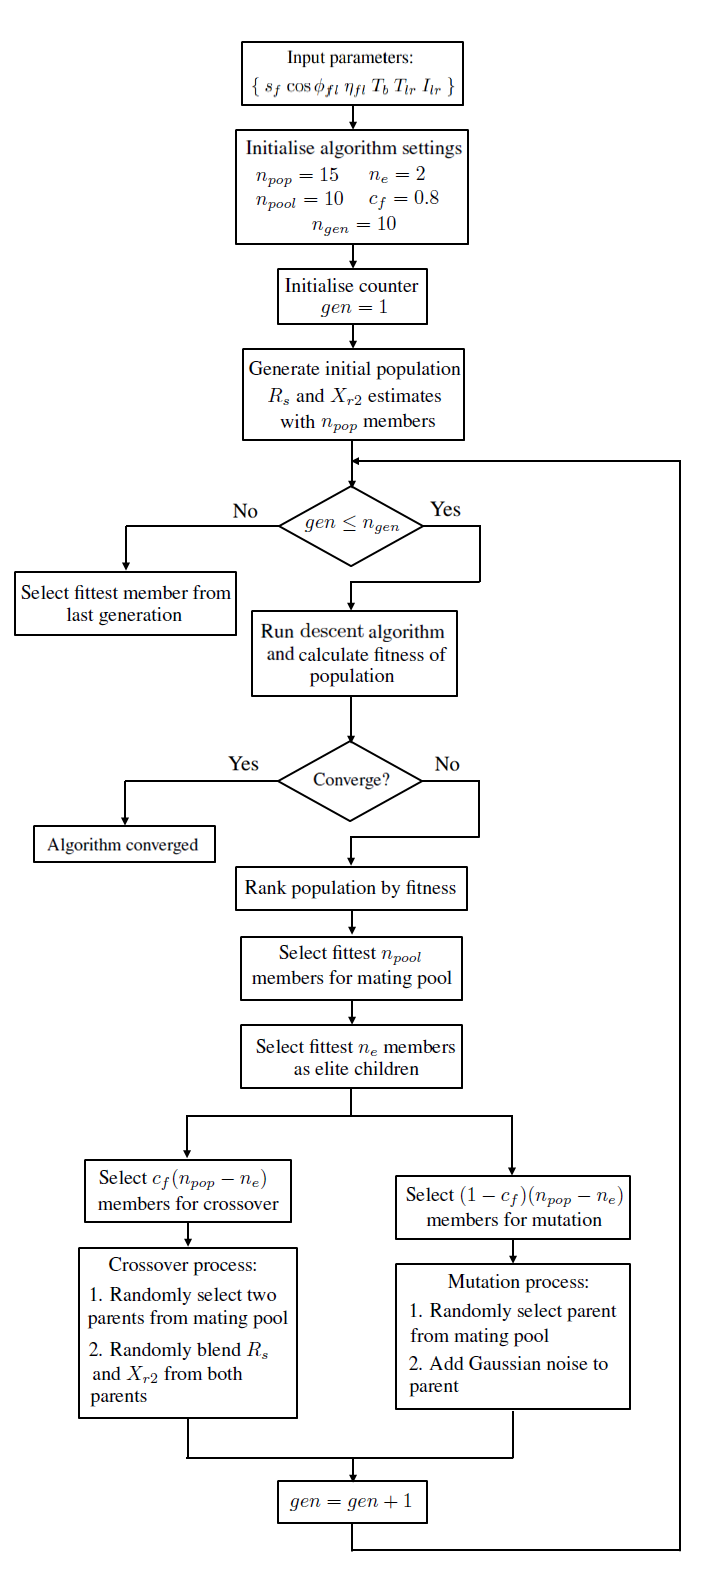
\includegraphics[scale=0.52]{./Figures/Hybrid_Algorithm.png}
\caption{Flowchart for hybrid algorithm (with natural selection of $R_{s}$ and $X_{r2}$)}
\label{fig:hybrid_algorithm}
\end{center}
\end{figure}

An initial population of $n_{pop}$ estimates for $R_s$ and $X_{r2}$ are randomly sampled from a uniform distribution with upper and lower limits as shown in Table \ref{tab:hybridga_range}. Each pair of estimates is referred to as a member of the population.

\begin{table}[!h]
	\renewcommand{\arraystretch}{1.3}
	\begin{center}
	\begin{tabular}{|c|c|c|}
        \hline
		  \multirow{2}{*}{Parameter} & \multicolumn{2}{|c|}{Range of Initial Estimate (pu)} \\ \cline{2-3}
        & Lower Bound & Upper Bound \\ \hline
        $R_{s}$  	& 0  & 0.15	\\ \hline
        $X_{r2}$  	& 0  & 0.15	\\ \hline
    \end{tabular}
	\caption{Range of initial parameter estimates}
	\label{tab:hybridga_range}
	\end{center}
\end{table}

The descent algorithm is then run on each member of the population. The fitness of each member (in terms of the squared error $\mathbf{F}'\mathbf{F}$) is calculated and ranked. The lowest fitness members are discarded and the rest are retained to form the mating pool for the next generation (there are $n_{pool}$ members in the mating pool).

The fittest $n_{e}$ members in the mating pool are retained for the next generation as \textbf{elite children}. Of the remaining $n_{pop} - n_{e}$ children to be created for the next generation, $c_{f}$\% will be produced by crossover and the rest ($1 - c_{f}$\%) by mutation. The proportion $c_{f}$ is called the \textbf{crossover fraction}.

\begin{enumerate}
\item \textbf{Crossover}: in the crossover process, two members of the mating pool are randomly selected and combined by taking a random blend of each member's parameters, e.g. the crossover of parameter $R_{s}$:

\begin{equation}
	R_{s, child} = \alpha R_{s, parent 1} + (1 - \alpha) R_{s, parent 2}
\end{equation}

\noindent where $\alpha$ is a random variable selected from a uniform distribution over the interval $[0,1]$

\item \textbf{Mutation}: in the mutation process, a member of the mating pool is randomly selected and its parameters are mutated by adding Gaussian noise with standard deviations of 0.01.
\end{enumerate}

The descent algorithm is then run for the next generation of estimates for $R_s$ and $X_{r2}$. The fitness is calculated and the process repeats itself for $n_{gen}$ generations. If at any point during the process the descent algorithm converges, then the hybrid algorithm stops and selects the parameter estimates from the converged descent algorithm as the solution. Otherwise, the parameter estimates yielding the best fitness after $n_{gen}$ generations are selected.

The recommended settings for the hybrid algorithm implemented in \textbf{Moto} are shown in Table \ref{tab:hybrid_default}. 

\begin{table}[htp]
	\renewcommand{\arraystretch}{1.3}
	\begin{center}
	\begin{tabular}{|c|c|c|}
        \hline
        Setting  	& Setting Description  & Default Value	\\ \hline
        $n_{pop}$  	& Population of each generation  & 15	\\ \hline
        $n_{pool}$  	& Number of members in the mating pool  & 10 \\ \hline
        $n_{e}$  	& Number of elite children  & 2	\\ \hline
        $c_{f}$  	& Crossover fraction  & 80\%	\\ \hline
        $n_{gen}$  	& Maximum number of generations  & 10	\\ \hline
    \end{tabular}
	\caption{Recommended settings for hybrid algorithm}
	\label{tab:hybrid_default}
	\end{center}
\end{table}

\newpage
\section{Using the Program}
\textbf{Moto} is quite straightforward to use. Simply fill in the details of the motor at the top the main screen (see Figure \ref{fig:moto_main}), select the model and algorithm settings and then press the"Calculate" button. The resulting equivalent circuit parameters will appear in per unit values at the bottom of the screen. The torque-speed and current-speed curves implied by the estimated parameters can then be viewed by pressing the "Plot" button (see Figure \ref{fig:moto_plot}).

\begin{figure}[!htp]
\begin{center}
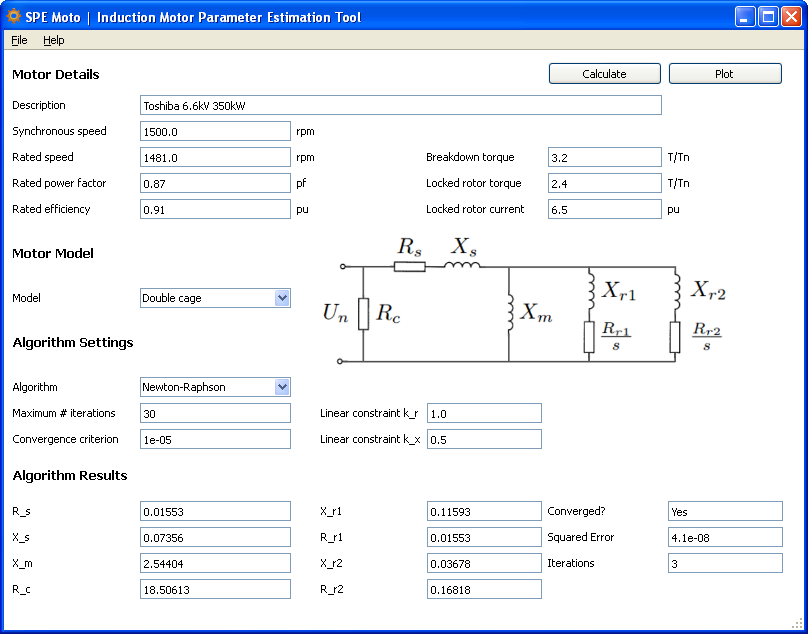
\includegraphics[scale=0.6]{./Figures/moto_main.png}
\caption{\textbf{Moto} main screen}
\label{fig:moto_main}
\end{center}
\end{figure}

\begin{figure}[!ht]
\begin{center}
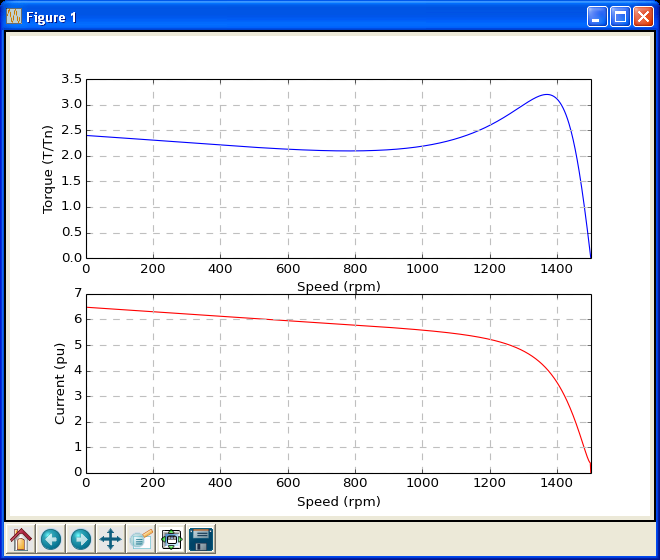
\includegraphics[scale=0.65]{./Figures/moto_plot.png}
\caption{\textbf{Moto} plotting function}
\label{fig:moto_plot}
\end{center}
\end{figure}

\subsection{Algorithm Settings}

\textbf{Algorithm:} select between the seven algorithms described in Section \ref{sec:algorithms}

\textbf{Maximum \# iterations:} is applicable to descent and hybrid algorithms and is the maximum number of iterations that the algorithm will execute without reaching convergence.

\textbf{Convergence criterion:} is the squared error value that the algorithms use as the convergence point. An algorithm will stop if it produces an estimate with a squared error below this covergence criterion. By default, the convergence criterion is $1 \times 10^{-5}$.

\textbf{Linear constraint k\_r:} is only applicable to descent algorithms. The linear constraint k\_r is the constant factor used to calculate the stator resistance $R_s$ (refer to Section \ref{sec:linear_constraints}).

\textbf{Linear constraint k\_x:} is only applicable to descent algorithms. The linear constraint k\_x is the constant factor used to calculate the outer cage rotor reactance $X_r2$ (refer to Section \ref{sec:linear_constraints}).

\textbf{Maximum \# generations:} is applicable to genetic and hybrid algorithms and is the maximum number of generations that the algorithm will evolve (refer to Section \ref{sec:genetic_algo}).

\textbf{Members in population:} is applicable to genetic and hybrid algorithms and is the number of members in each generation of estimates (refer to Section \ref{sec:genetic_algo}).

\textbf{Members in mating pool:} is applicable to genetic and hybrid algorithms and is the number of members that are retained for mating in each generation (refer to Section \ref{sec:genetic_algo}).

\textbf{Elite children:} is applicable to genetic and hybrid algorithms and is the number of elite children that will be spawned for each generation (refer to Section \ref{sec:genetic_algo}).

\textbf{Crossover fraction:} is applicable to genetic and hybrid algorithms and is the number of children that will be created through the crossover process (refer to Section \ref{sec:genetic_algo}).

\subsection{Algorithm Results}

\textbf{R\_s:} is the stator resistance (in per unit)

\textbf{X\_s:} is the stator reactance (in per unit)

\textbf{X\_m:} is the magnetising reactance (in per unit)

\textbf{R\_c:} is the core loss resistance (in per unit)

\textbf{X\_r1:} is the inner cage rotor reactance (in per unit)

\textbf{R\_r1:} is the inner cage rotor resistance (in per unit)

\textbf{X\_r2:} is the outer cage rotor reactance (in per unit)

\textbf{R\_r2:} is the outer cage rotor resistance (in per unit)

\textbf{Converged:} is a Yes / No status indicating whether the algorithm has converged.

\textbf{Squared Error:} is the resulting squared error of the algorithm

\textbf{Iterations:} is the number of iterations (or generations) that the algorithm executed

\subsection{Saving and Loading}
\textbf{Moto} can save and load otor data using the "Save as..." and "Open File..." items respectively in the File menu. The motor details and algorithm settings are saved in the \textbf{Moto} data files. Note that algorithm results are not saved and need to be re-calculated.

\subsection{Plotting}
The torque-speed and current-speed curves of the motor can be shown by pressing the "Plot" button. The resulting figure can be panned, zoomed and saved as an image using the toolbar at the bottom of the dialog box.

\newpage
\section{Troubleshooting}
\subsection{Algorithm Not Converging}
Not all motors have a convergent solution. In some cases, the motor's performance cannot be characterised by a single cage or double cage model with constant parameters. In such cases, the best approximation is desired and this is application-dependent. For example, if a motor starting study is required, then a more accurate representation of the motor's starting characteristics is more important than high accuracy at low slip values. Thus the motor parameters can be tuned to result in better starting performance while perhaps sacrificing accuracy at motor breakdown. 

In other cases, a valid solution exists, but the selected algorithm is not reaching it. Here, the squared error value is an important guide to check whether changes in algorithms and settings are having a positve or negative effect. 

Based on our experience, we recommend the following general workflow for solving induction motor parameter estimation problems using double cage models:

\begin{enumerate}
\item As an initial attempt, use the conventional Newton-Raphson algorithm with fixed linear constraints $k_{r} = 1$ and $k_{x} = 0.5$
\item If there is no convergence, use the damped NR algorithm with fixed linear constraints $k_{r} = 1$ and $k_{x} = 0.5$
\item If there is no convergence, try the LM algorithm with fixed linear constraints $k_{r} = 1$ and $k_{x} = 0.5$
\item If there is no convergence, try the hybrid DNR-GA algorithm
\item If there is no convergence, try the hybrid LM-GA algorithm
\item Finally, if there is still no convergence, use the genetic algorithm with 50 to 100 generations to give a solution with an adequately low squared error value
\end{enumerate}

\subsection{Bugs}
If you find a bug in the software, please send us a mesasge at \href{mailto:contact@sigmapower.com.au}{contact@sigmapower.com.au}.

% Bibliography
\newpage
\bibliographystyle{plain}
\bibliography{bib_refs}

\end{document}
